\lhead{\emph{Methodology}}

% ***************************************************************************
\chapter{Methodology}
% ***************************************************************************

\section{Environment}

    As explained previously (\ref{int:chall}), the purpose of this work is to compare registration techniques in a specific case where point cloud registration is challenging. I realized a benchmark of methods described in the section \ref{ch:soa} and the modified one detailed in section \ref{chapt:implementation}. Each method is compared in different scenarios ; registering point clouds acquired from our real sensors in the kitchen scene, performing the registration on the kitchen with simulation data and finally with common point cloud databases to compare with the results from literature. 

    \subsection{Real scenario}

        Our real scenario is composed by 2 kinects filming a kitchen counter top and shelves filled with common kitchen objects. \\
        In this scenario on e of the main point is to define accurately the ground truth, is is possible to measure with few mm of error the translation between cameras but their relative orientation is much more difficult to measure. To evaluate this ground truth as accurately as possible I used all the knowledge we have: defining the initial guess as the manually measured translation and assuming equal orientation (cameras are facing in the same direction). I then align point clouds more accurately with the plane detection method and finely adjust the transform by hand so that point clouds match exactly.

    \subsection{Simulation}\label{subsec:simulation}
    
    Using 3D models of kitchen furnitures, I recreated the scene inside gazebo simulator which is compatible with \acrshort{ros} and I was able to publish point clouds topic using simulated kinects sensors. This setup is then working exactly in the same way as the previous one, our program can subscribe and share point cloud topics through \acrshort{ros}. \\
    In this case the ground truth is perfectly know as it is defined inside the gazebo world model where I placed the sensors with absolute coordinates and orientation.

\section{Variables}

    The objective of the algorithm is to estimate the transform between two kinects, I then need to compare this transform (rotation and translation) with the ground truth. It is difficult to find a meaningful scalar metric to compare transform matrices. We can nevertheless compare separately translation and rotation parts, by computing the overall translation distance $l$ and rotation angle $\theta$ around the fix axis $a$.
    Let $\mathcal{T}$ be the $4\times 4$ homogeneous matrix with rotation part described by coordinates of basis vectors $u, v, w$  the target frame written in the source frame and $t$ the translation vector between both frames' origins (fig. \ref{fig:transf}).
    \[
        \begin{bmatrix}
            u_x & v_x & w_x & t_x\\ 
            u_y & v_y & w_y & t_y\\ 
            u_z & v_z & w_z & t_z\\ 
            0 & 0 & 0 & 1
        \end{bmatrix}
    \]
    
    \begin{figure}[h!]
        \centering
        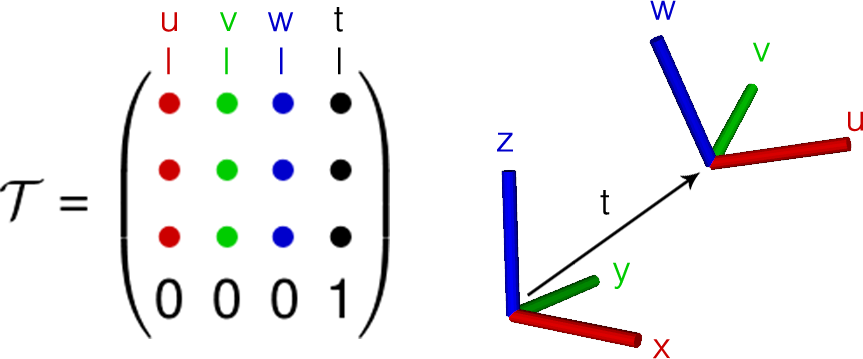
\includegraphics[width=\textwidth]{images/transform.png}
        \caption{Transform matrix description. \\
        $\mathcal{T}$ describes the transform between $xyz$ and $uvw$.}
        \label{fig:transf}
    \end{figure}
    
    We'll describe this transform with the following two metrics.
    
    \begin{equation} \label{eq:tf_transl_comp}
        \left.
        \begin{aligned}
        l(\mathcal{T}) &
        =   \begin{Vmatrix}
                t
            \end{Vmatrix} \\
         &
            = \sqrt{t_x^2+t_y^2+t_z^2}
        \end{aligned}
     \right\}
     \qquad \text{the translation metric}
    \end{equation}
    
    Using the fact that the rotation axis is 
    \[
        \mathbf{a}=\begin{pmatrix}
        w_y-v_z \\
        u_z-w_x \\
        v_x-u_y \\
        \end{pmatrix}^T
    \]
    with
    \[
        \begin{Vmatrix}
        \mathbf{a}
        \end{Vmatrix}
        =2sin(\theta)
    \]
    and 
    \[
        Tr(R) = 1 + 2\cos \theta
    \]
    We can compute the rotation angle from the matrix coefficients:
    \begin{equation} \label{eq:tf_rot_comp}
        \left.
        \begin{aligned}
        \theta(\mathcal{T}) &
        = \arctan \left( \frac{\sqrt{(w_y-v_z)^2 + (u_z-w_x)^2 + (v_x-u_y)^2 }}{u_x + v_y + w_z - 1} \right)
        \end{aligned}
     \right\}
     \qquad \text{the rotation metric}
    \end{equation}
